\subsection{Расчет характеристик манёвренности самолета}
\label{sec:Расчёт характеристик манёвренности самолёта}
\pagestyle{fancy}
\fancyhf{}
\rhead{Дипломная работа}
\lhead{Расчёт манёвренных характеристик}
\rfoot{\thepage}

\subsubsection{Расчетные формулы и соотношения}

Для неманёвренного самолёта характеристики предельного правильного виража расчитываются для высоты $H = 6$км.

Характеристики маневренности рассчитываются при 50\%-ом выгорании топлива для
массы самолета: 

\begin{equation}
    \label{eq:Относительная масса смолёта}
    \bar{m}_c = 1-0,5\bar{m}_\text{т}
\end{equation}

Максимально допустимая нормальная перегрузка -- 
\begin{equation}
    \label{eq:Максимально допустимая нормальная перегрузка}
    n_{y_\text{доп}} = min \{n_{y_\text{э}},n_{y}(C_{y_\text{доп}}) \}
\end{equation}

\begin{equation}
    \label{eq:Эксплуатационная перегрузка}
    n_{y_\text{э}} = 2,5...3,5
\end{equation}

Допустимая нормальная перегрузка -- 
\begin{equation}
    \label{eq:Допустимая нормальная перегрузка}
    n_{y_\text{э}} = \frac{C_{y_\text{доп}}}{C_{y_\text{ГП}}}
\end{equation}

Коэффициент подъёмной силы горизонтального полёта --
\begin{equation}
    \label{eq:Коэффициент подъёмной силы горизонтального полёта}
    C_{y_\text{ГП}} = \frac{\bar{m}_cP_s10}{q}
\end{equation}

Нормальная перегрузка на вираже --
\begin{equation}
    \label{eq:Нормальная перегрузка на вираже}
    n_{y_\text{вир}} = min \{ n_{y_\text{доп}}, n_{y_P} \}
\end{equation}

Нормальная перегрузка горизонтального полёта -- 
\begin{equation}
    \label{eq:Нормальная перегрузка горизонтального полёта}
    n_{y_P} = \frac{1}{C_{y_\text{ГП}}} \sqrt{\frac{\bar{P}C_{y_\text{ГП}}-C_{x_0}}{A}},
\end{equation}
где $$\bar{P} = \frac{P_\text{р}}{mg}$$

Угловая скорость при предельном правильном вираже --
\begin{equation}
    \label{eq:Угловая скорость при предельном правильном вираже}
    \omega_\text{вир} = \frac{g}{V}\sqrt{n^2_{y_\text{вир}}-1}
\end{equation}

Радиус предельного правильного виража -- 
\begin{equation}
    \label{eq:Радиус предельного правильного виража}
    r_\text{вир} = \frac{V}{\omega_\text{вир}}
\end{equation}

Время выполнения предельного правильного виража -- 
\begin{equation}
    \label{eq:Время выполнения предельного правильного виража}
    t_\text{вир} = \frac{2\pi r_\text{вир}}{V}
\end{equation}

\subsubsection{Результаты расчета}
\label{sec:Результаты расчётов манёвренности самолёта}


\begin{longtable}[H]{|c|c|c|c|c|c|c|c|c|c|}
    \caption{Итоговая таблица} \label{tab:Результаты Манёвры} \\
    \hline 
    $M$ & $V$, м/c & $n_{y_P}$ &  $n_{y_\text{ГП}}$ & $n_{y_\text{доп}}$ & $n_{y_\text{вир}}$& $\omega_\text{вир}$, 1/с & $r_\text{вир},$ м & $t_\text{вир}$ \\ \hline
    \endfirsthead
    
    \multicolumn{10}{c}%
    {{ \tablename\ \thetable{}: Итоговая таблица}} \\
    \hline 
    $M$ & $V$, м/c & $n_{y_P}$ & $n_{y_\text{ГП}}$ & $n_{y_\text{доп}}$ & $n_{y_\text{вир}}$& $\omega_\text{вир}$, 1/с & $r_\text{вир},$ м & $t_\text{вир}$  \\ \hline
    \endhead
    \endfoot
    
    \hline \hline
    \endlastfoot
    \hline
    0.41 & 129.81 & 3.027 & 1.104 & 1.049 & 1.049 & 0.02384 & 5443.8 & 263.4 \\ \hline 0.51 & 161.47 & 3.649 & 1.711 & 1.626 & 1.626 & 0.07788 & 2073.1 & 80.6 \\ \hline 0.61 & 193.13 & 4.252 & 2.456 & 2.334 & 2.334 & 0.1071 & 1803.2 & 58.6 \\ \hline 0.71 & 224.79 & 4.815 & 3.305 & 3.14 & 3.14 & 0.12989 & 1730.6 & 48.3 \\ \hline 0.81 & 256.45 & 5.286 & 4.176 & 3.5 & 3.5 & 0.12831 & 1998.7 & 48.9 \\ \hline 0.91 & 288.11 & 5.589 & 5.021 & 3.5 & 3.5 & 0.11421 & 2522.7 & 55.0 \\ \hline 1.01 & 319.77 & 5.626 & 5.896 & 3.5 & 3.5 & 0.1029 & 3107.6 & 61.0 \\ \hline 1.11 & 351.43 & 5.225 & 6.898 & 3.5 & 3.5 & 0.09363 & 3753.4 & 67.1 \\ \hline 1.21 & 383.09 & 3.941 & 8.009 & 3.5 & 3.5 & 0.08589 & 4460.1 & 73.1 \\ \hline 1.31 & 414.75 & - & 9.136 & 3.5 & 3.5 & 0.07933 & 5227.8 & 79.2
        
\end{longtable}

\begin{figure}[H]
    \center{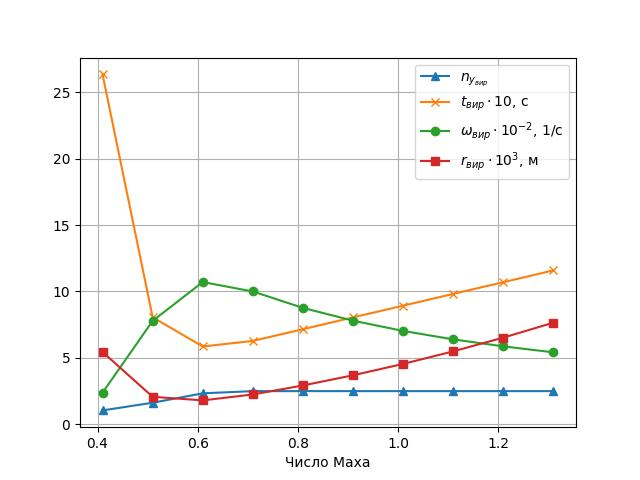
\includegraphics[width=\linewidth]{Оглавление/Part1/figures/РезультатыМаневры.jpg}}
    \caption{Характеристики правильного предельного виража }
    \label{fig:image}
\end{figure}

\begin{figure}[H]
    \center{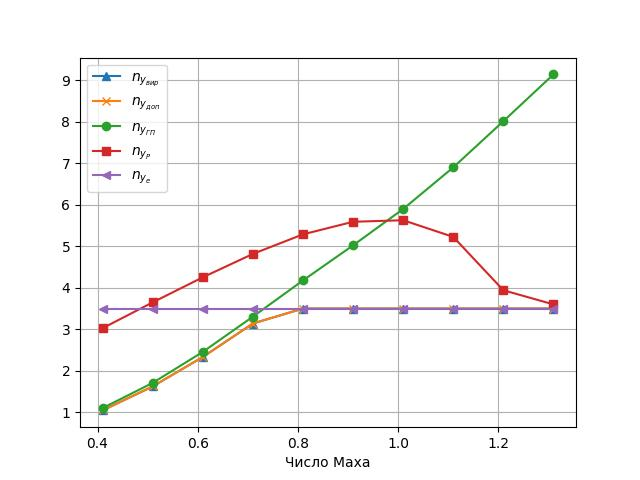
\includegraphics[width=\linewidth]{Оглавление/Part1/figures/РезультатыМаневры2.jpg}}
    \caption{Перегрузки при выполнении виража}
    \label{fig:image}
\end{figure}

\begin{center}
    Выводы:
\end{center}

В ходе расчетов в данном разделе были получены следующие результаты:
\begin{itemize}
    \item [-] угловая скорость виража изменяется от 0,024 $\frac{1}{c}$ до 0,08 $\frac{1}{c}$ на диапазоне
чисел М, при которых возможен правильный предельный вираж на высоте 6 км
    \item [-] радиус виража изменяется в диапазоне от 5443,8 м до 5227,8 м
    \item [-] время выполнения виража изменяется в диапазоне от 263,3 с до 79,2 с
\end{itemize}
По полученным данным можно сказать, что самолет –прототип Concorde обладает
довольно хорошими характеристиками предельного правильного виража





